
Se desea trabajar con series temporales sobre mediciones climatológicas. 
En concreto, se eligen las variables de temperatura del aire, humedad relativa y presión atmosférica en la superficie.
Dichas variables son estudiadas con frecuencia horaria, en el intervalo comprendido entre el 1 de marzo de 2023 y el 28 de febrero de 2025.

Es imprescindible disponer de un conjunto de datos que abarque un período de tiempo suficientemente amplio para poder cubrir las diversas condiciones climáticas que pueden presentarse.
Además, es relevante el uso de datos en un período múltiplo del año, para asegurar que se capturan las variaciones estacionales y que el conjunto de datos está suficientemente equilibrado.
Es decir, si se emplearan un año y 3 meses, se podría sesgar el conjunto introduciendo más días con temperaturas bajas, por ejemplo, si se cubrieran 2 inviernos pero un solo verano.

\section{Fuentes de los datos}

Se han empleado 2 fuentes para recopilar las mediciones: 
\begin{itemize}
    \item \textbf{Grafcan}: Cartográfica de Canarias, S.A. es una empresa pública de la Comunidad Autónoma de Canarias. Dispone de una red de estaciones meteorológicas cuyas
    mediciones son accesibles mediante una API REST de acceso gratuito previa solicitud de una clave\cite{grafcan_sensores}. 
    \item \textbf{Open-Meteo}: API pública de código abierto que proporciona datos de múltiples proveedores de meteorología. Este servicio no dispone de estaciones de medición
    propias, sino que recopila pronósticos de diferentes modelos de predicción climatológica. 

    Se emplea la API de predicciones pasadas\cite{open_meteo_api}. Se seleccionan los modelos ICON Global del servicio meteorológico alemán (DWD) y el modelo ARPEGE Europe de Météo-France. Ambos modelos se actualizan cada 3 horas. 
    Se explora la posibilidad de emplear as predicciones del modelo HAROME de la AEMET, pero no están disponibles de forma pública
\end{itemize}

Se eligen 4 ubicaciones de la isla de Tenerife con distintas características climáticas para el conjunto de entrenamiento y evaluación:
\begin{itemize}
    \item \textbf{San Cristóbal de La Laguna 1 (A)}: La Cuesta, 35 metros de altitud.
    \item \textbf{San Cristóbal de La Laguna 2 (B)}: La Punta del Hidalgo, 54m.
    \item \textbf{La Orotava (C)}: Camino de Chasna, 812m.
    \item \textbf{Arona (D)}: Punta de Rasca, 25m.
\end{itemize}

Así mismo, se escogen 2 ubicaciones para el conjunto de test, nunca vistas en el ajuste del modelo:
\begin{itemize}
    \item \textbf{Garachico (E)}: La Montañeta, 922 m.
    \item \textbf{Santa Cruz de Tenerife (F)}: Polígono Costa Sur, 92m.
\end{itemize}

Las ubicaciones han sido elegidas al contar con estaciones de medición de Grafcan.
Sus posiciones se muestran en la Figura \ref{mapa_estaciones}, con la letra indicada en la lista.
Se señaladan en rojo las estaciones de entrenamiento y en naranja las de test.

\begin{figure}[htb]
   \centering
   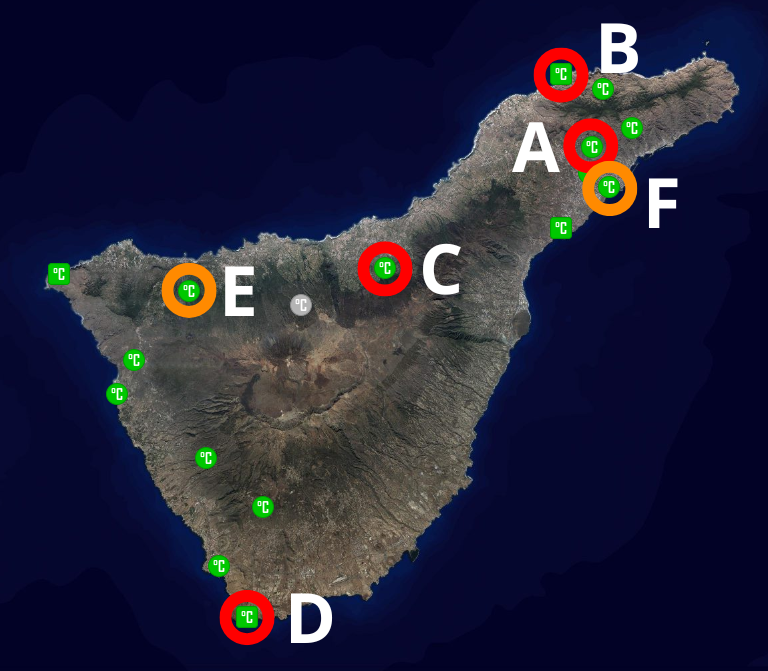
\includegraphics[width=0.6\linewidth]{images/mapa_estaciones}
   \caption{Mapa de las estaciones climatológicas Grafcan empleadas.}
   \label{mapa_estaciones}
\end{figure}

Inicialmente se valoró emplear las estaciones correspondientes a Los Cristianos, Santiago del Teide o la Punta de Teno, pero fueron descartadas por dos motivos: 
se detectó que existían períodos prolongados con datos faltantes en las mediciones de Grafcan. Algunas de ellas también exhibían poca correlación entre las mediciones
del servicio Grafcan y las de Open-Meteo, lo que podría afectar la calidad de los datos.

\bigskip

\section{Proceso de adquisición y almacenamiento}

Para automatizar la adquisición de datos, se emplea la herramienta de orquestación node-red, que permite crear flujos de información mediante nodos que realizan tareas específicas o ejecutan códgio de JavaScript.
En dicha herramienta se desarrollan dos paneles, uno para cada fuente de datos. 
Así mismo, dentro de cada panel se desarrollan dos flujos, uno para la adquisición de datos en un intervalo dado, y otro para la adquisición de datos en tiempo real, en particular, 
se establece la recogida de datos cada 6 horas.

\subsection{Flujos de adquisición de Grafcan}
Debido al funcionamiento de la API de Grafcan, se debe realizar una llamada para obtener la serie temporal de cada variable meteorológica de cada estación.
Posteriormente, se unen las series de cada estación en una única serie, que se almacena en una base de datos PostgreSQL. Este flujo está reflejado en la figura \ref{grafcan_flows}.
\begin{figure}[htb]
   \centering
   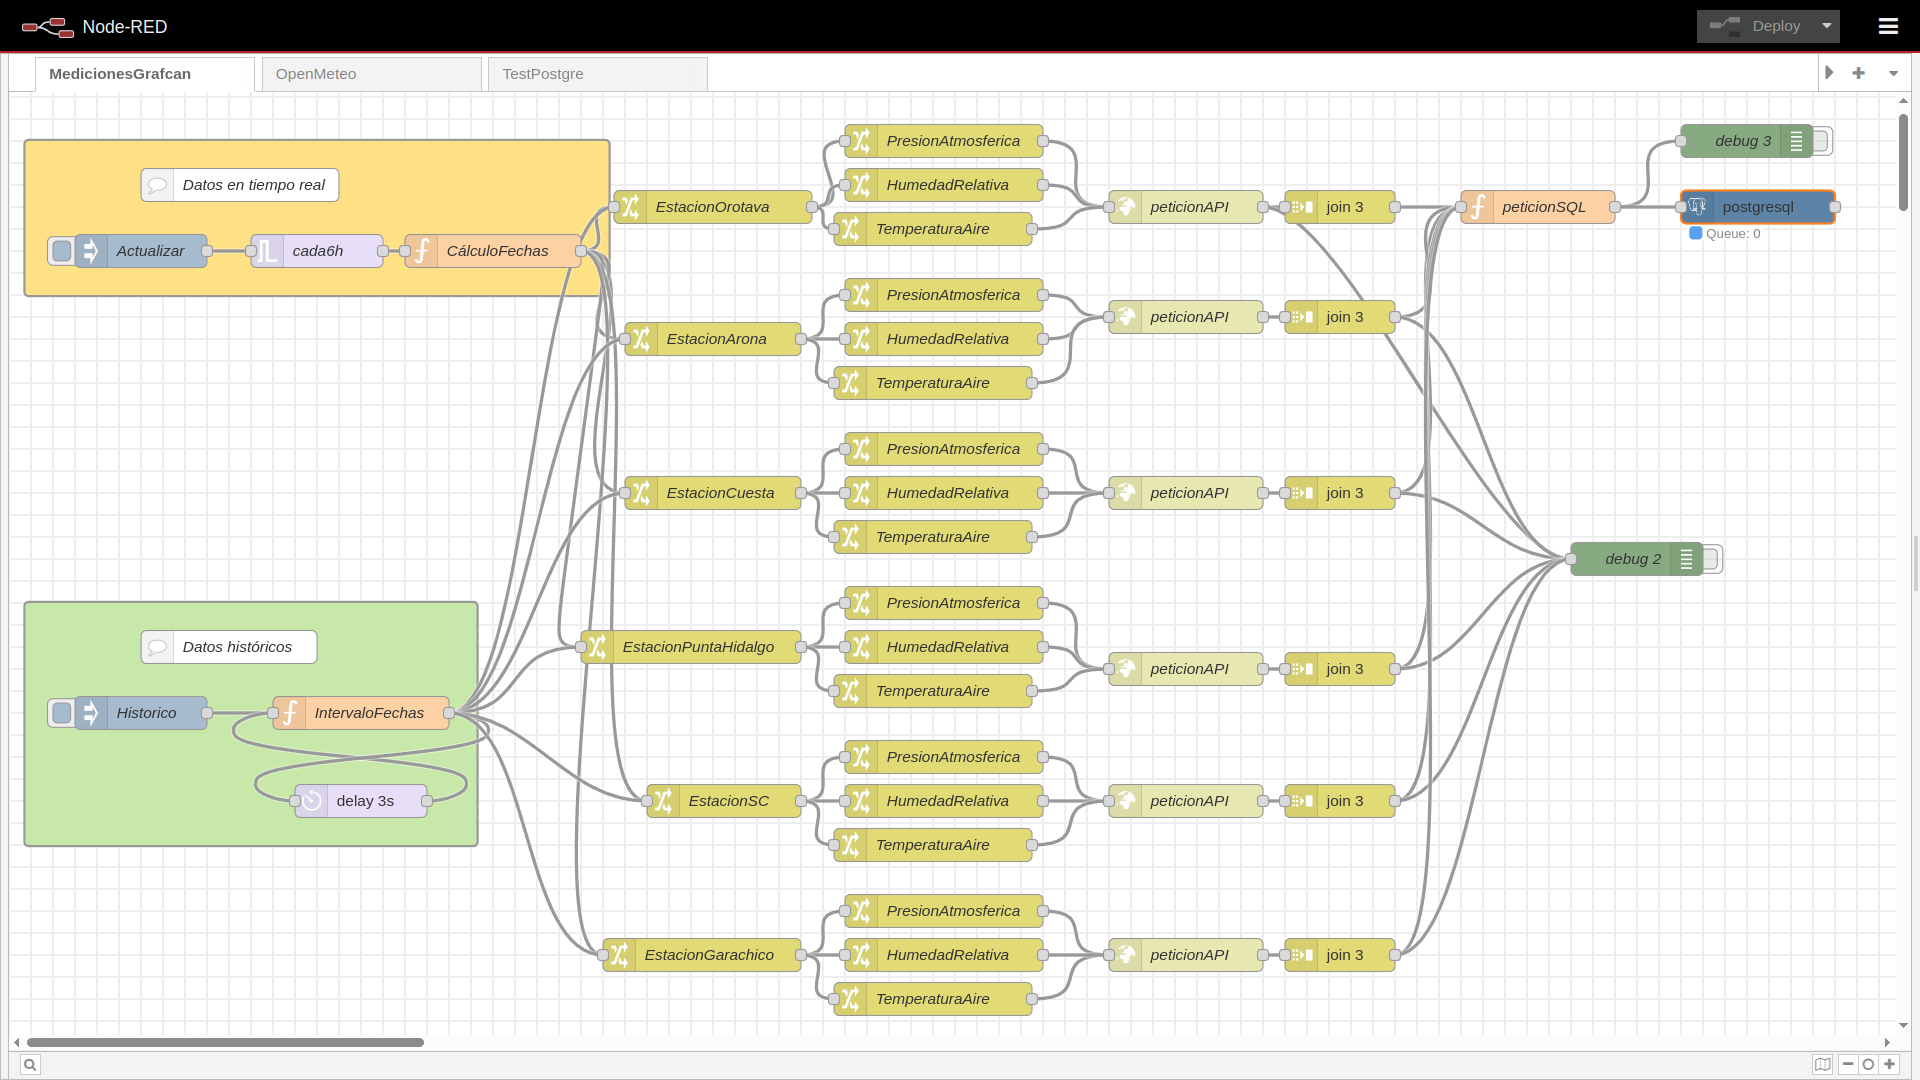
\includegraphics[width=1\linewidth]{images/node-red_grafcan.png}
   \caption{Flujo de adquisición de datos de Grafcan en node-red.}
   \label{grafcan_flows}
\end{figure}

Las mediciones de Grafcan se recogen apróximamente cada 10 minutos, si bien la frecuencia no es consistente y en ocasiones es mayor. Así mismo, 
los instantes de medición son independientes entre las variables estudiadas. Para manejar esta variabilidad, 
en este nivel los datos se agregan cada 10 minutos, usando la media de las mediciones del intervalo.

\subsection{Flujos de adquisición de Open-Meteo}
Existe una rama para obtener los datos del modelo ICON y otra para el modelo ARPEGE. Se establecen las coordenadas de cada ubicación como las de la estación de Grafcan seleccionada 
y se realiza una llamada a la API por cada localización y cada modelo, como se observa en la figura \ref{open-meteo_flows}. 
Los resultados se almacenan en una base de datos PostgreSQL.
\begin{figure}[htb]
   \centering
   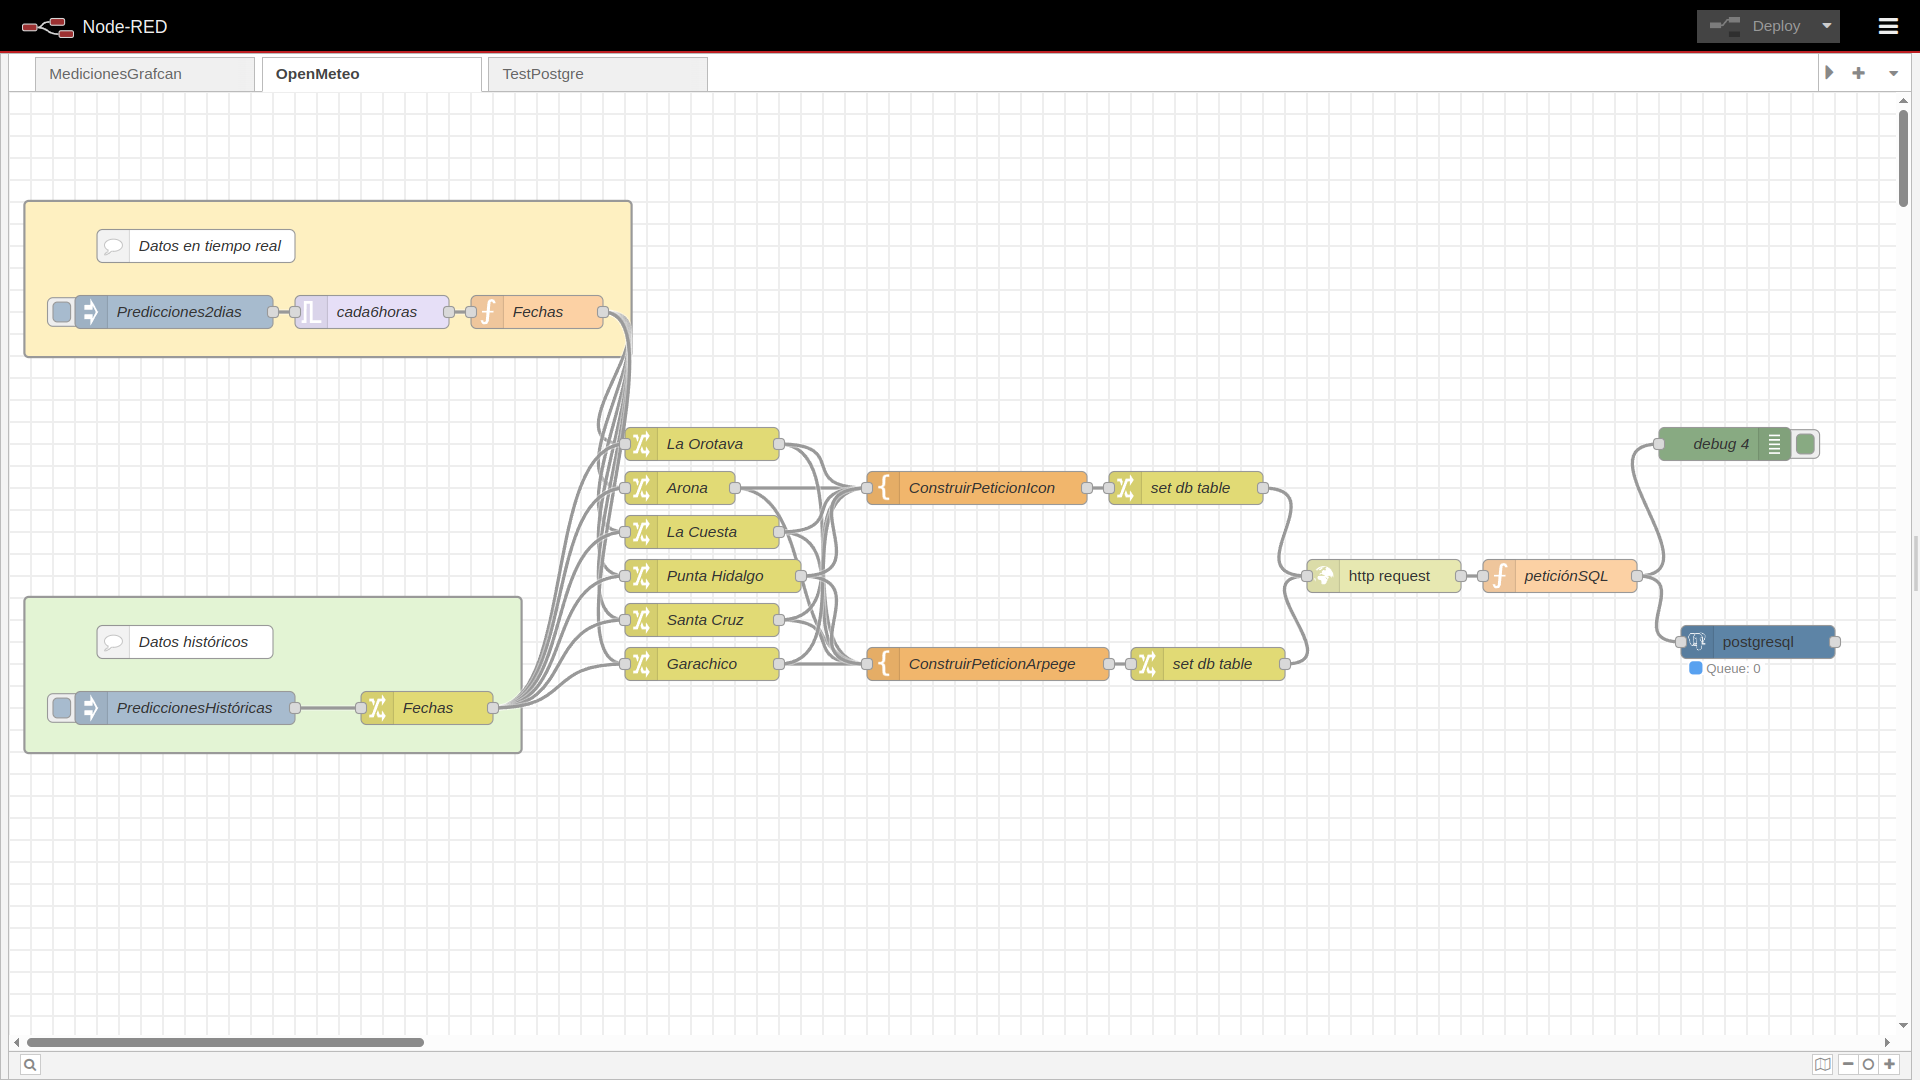
\includegraphics[width=1\linewidth]{images/node-red_open-meteo.png}
   \caption{Flujo de adquisición de datos de Open-Meteo en node-red.}
   \label{open-meteo_flows}
\end{figure}

\subsection{Almacenamiento}
Se estudian distintas alternativas para el almacenamiento de los datos, fundamentalmente, servicios de bases de datos como Redis, MongoDB o PostgreSQL.
Tras valorar las opciones, se opta por emplear TimescaleDB, una extensión del popular sistema PostgreSQL
de bases de datos relacionales, especialmente adaptada para el manejo de series temporales. 

Se establece un servidor TimescaleDB en un contenedor Docker. Se configura una tabla para cada estación y cada fuente: Grafcan, Open-Meteo ICON y Open-Meteo ARPEGE. 
Cada tabla emplea como índice y clave primaria la fecha y hora de la medición, así como su zona horaria. Las otras columnas se corresponden a la temperatura media del aire
 en grados Celsius, la humedad relativa en porcentaje y la presión atmosférica en superficie medida en hPa.

Es importante señalar que las mediciones de Grafcan y Open-Meteo codifican las horas en UTC, en vez de la hora local, puesto que UTC es independiente a los cambios de horario
y de esta forma se mantiene la consistencia de los datos.

\section{Preprocesado}

Se desarrolla un cuaderno de Jupyter para realizar el preprocesado de los datos. El proceso descrito en este apartado
se aplica de forma separada para cada ubicación.

En primer lugar, se obtienen las series temporales de las 3 fuentes: Grafcan y los dos modelos de Open-Meteo, para el período entre el 1 de marzo de 2023 y el 28 de febrero de 2025.
Se agregan los datos con frecuencia horaria mediante la media. 

\textbf{Nota:} En la estación de Garachico, usada para el test, el período empleado es del 1 de marzo de 2024 al 28 de febrero de 2025, puesto que el período de 2023 tiene 
un gran número de datos faltantes.

\subsection{Visualización}
Se visualizan los datos de cada variable para cada año. Podemos ver ejemplos en las figuras \ref{visualizacion_1}, \ref{visualizacion_2} y \ref{visualizacion_3}.

Se observa claramente que en la presión atmosférica las mediciones de todas las fuentes son muy similares. Sin embargo, 
en la temperatura del aire y la humedad relativa se aprecian diferencias entre las distintas fuentes.
\begin{figure}
    \centering
    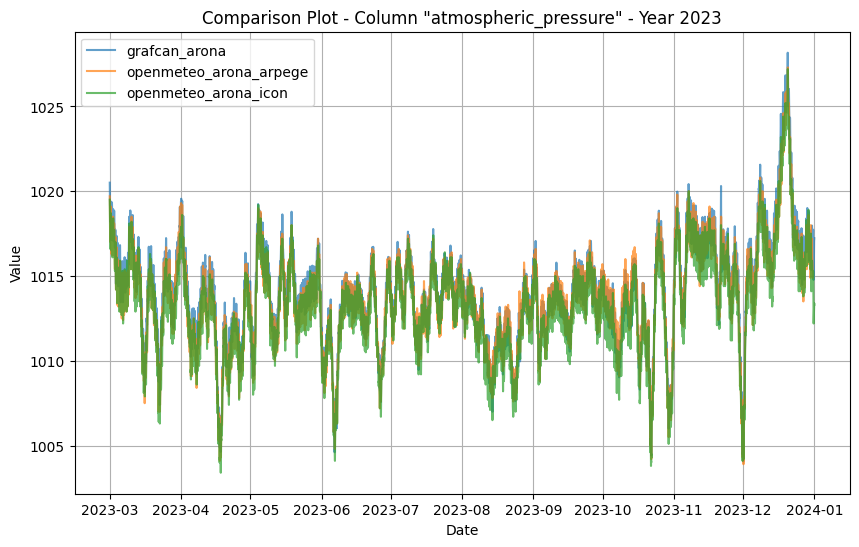
\includegraphics[width=.8\linewidth]{images/visualizacion_1.png}
    \caption{Visualización de la presión atmosférica en Arona durante 2023.}
    \label{visualizacion_1}
\end{figure}
\begin{figure}
    \centering
    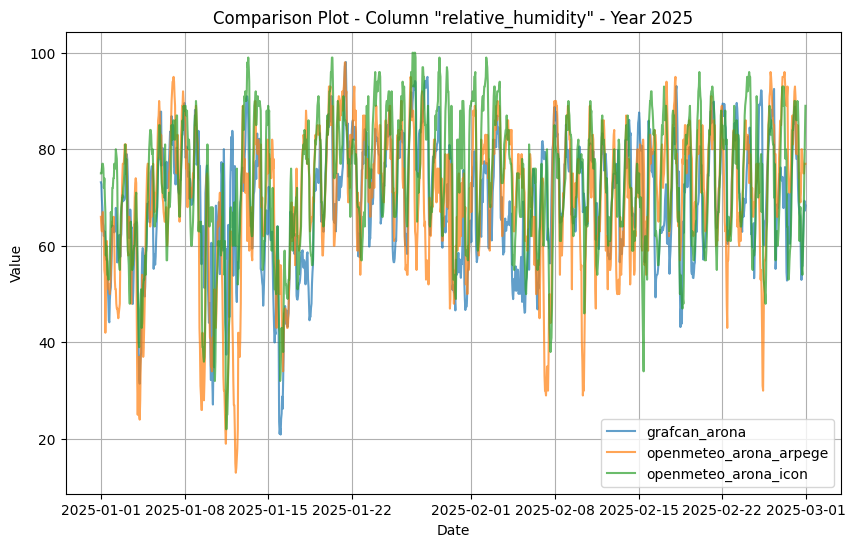
\includegraphics[width=.8\linewidth]{images/visualizacion_2.png}
    \caption{Visualización de la temperatura del aire en Arona durante 2024.}
    \label{visualizacion_2}
\end{figure}
\begin{figure}
    \centering
    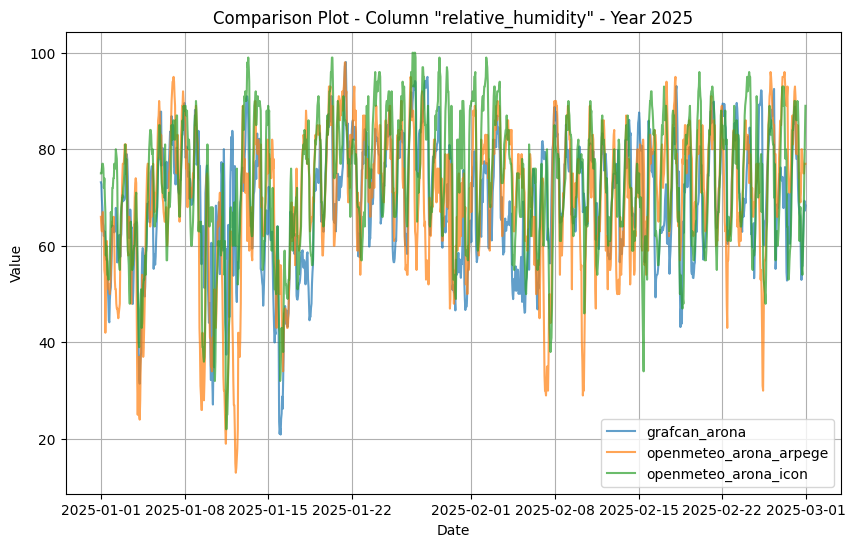
\includegraphics[width=.8\linewidth]{images/visualizacion_3.png}
    \caption{Visualización de la humedad relativa en Arona durante 2025.}
    \label{visualizacion_3}
\end{figure}

Cabe destacar que en la variable de humedad relativa se observa una gran variabilidad entre los datos de las distintas fuentes, que se constatará más adelante.

\subsection{Manejo de datos faltantes}
Se detectan los datos faltantes para cada fuente. Las estadísticas se muestran en la tabla \ref{tabla_datos_faltantes}. 
Es reseñable que el modelo ICON no muestra datos faltantes, mientras que el modelo ARPEGE tiene 35 horas faltantes consecutivas, en el período entre el 31 de diciembre de 2023 y el 1 de enero de 2024.

\begin{table}[htb]
    \small
    \centering
    \begin{tabular}{|c|c|c|c|}
        \hline
        Estación & Grafcan & Open-Meteo ICON & Open-Meteo ARPEGE \\
        \hline
        La Laguna 1 (La Cuesta) & 47 & 0 & 35 \\
        La Laguna 2(La Punta del Hidalgo) & 30 & 0 & 35 \\
        La Orotava & 3 & 0 & 35 \\
        Arona & 17 & 0 & 35 \\
        Garachico & 5 & 0 & 0 \\
        Santa Cruz de Tenerife & 0 & 0 & 46 \\
        \hline
    \end{tabular}
    \caption{Datos faltantes por estación y fuente de datos (en horas)}
    \label{tabla_datos_faltantes} 
\end{table}

Se decide imputar los datos faltantes mediante un método híbrido: si una secuencia de datos faltantes es menor a 5 horas se emplea 
un método de interpolación cúbica por tramos denominado PCHIP\cite{fritsch1980}, que preserva la forma de los datos y evita oscilaciones indeseadas.
Si la secuencia de datos faltantes es mayor a 5 horas, se copian los datos del día anterior en las mismas horas. 
Este tipo de imputación es común en el ámbito de las series temporales \cite{tawakuli2024}.

Los datos sintéticos son etiquetados como tales para poder ser identificados posteriormente.


\subsection{Selección de modelo de Open-Meteo}
Para cada variable se selecciona el modelo de Open-Meteo que mejor se ajusta a los datos de Grafcan.
Se emplean diversas métricas: los coeficiente de correlación de Pearson, Spearman y Kendall, así como el error cuadrático medio (MSE) y 
la distancia euclídea. Se elige el modelo que mejor resultados da en la mayoría de indicadores. Los modelos seleccionados y un ejemplo de las métricas
 se muestran en las tablas \ref{tabla_modelos_seleccionados} y .

\begin{table}[htb]
    \centering
    \begin{tabular}{|c|c|c|c|}
        \hline
        Estación & Temperatura del aire & Presión atmosférica & Humedad relativa \\
        \hline
        La Laguna 1 & ICON & ARPEGE & ICON \\
        La Laguna 2 & ARPEGE & ARPEGE & ARPEGE \\
        La Orotava & ICON & ARPEGE & ICON \\
        Arona & ICON & ARPEGE & ICON \\
        Garachico & ICON & ICON & ICON \\
        Santa Cruz de Tenerife & ICON & ARPEGE & ICON \\
        \hline
    \end{tabular}
    \caption{Modelo de Open-Meteo seleccionado para cada variable y estación}
    \label{tabla_modelos_seleccionados}
\end{table}

\begin{table}[h!]
\centering
\caption{Métricas de similitud con Grafcan para Arona}
\label{tab:sim_metrics}
\footnotesize {
\begin{tabular}{l  cc  cc  cc}
\toprule
\textbf{Métrica} &
\multicolumn{2}{c}{\textbf{air\_temperature}} &
\multicolumn{2}{c}{\textbf{atmospheric\_pressure}} &
\multicolumn{2}{c}{\textbf{relative\_humidity}} \\
\cmidrule(lr){2-3} \cmidrule(lr){4-5} \cmidrule(lr){6-7}
 & \textbf{ICON} & \textbf{ARPEGE} & \textbf{ICON} & \textbf{ARPEGE} & \textbf{ICON} & \textbf{ARPEGE} \\
\midrule
Pearson               & 0.8871 & 0.8415 & 0.9890 & 0.9891 & 0.6281 & 0.3838 \\
Spearman              & 0.9116 & 0.8519 & 0.9859 & 0.9866 & 0.6026 & 0.2748 \\
Kendall               & 0.7489 & 0.6650 & 0.9048 & 0.9070 & 0.4423 & 0.1973 \\
MSE                   & 2.8616 & 5.6179 & 1.1085 & 0.5754 & 208.6453 & 406.1746 \\
Euclidean Distance    & 224.0627 & 313.9447 & 139.4523 & 100.4768 & 1913.2363 & 2669.4431 \\
\bottomrule
\end{tabular}
}
\end{table}


Observamos que, en general, el modelo ICON es el que mejor se ajusta a las variables de temperatura del aire y humedad relativa,
 mientras que el modelo ARPEGE es el que mejor se ajusta a la presión atmosférica.

 Resulta reseñable señalar que la diferencia entre los modelos de Open-Meteo y Grafcan es mucho mayor en la variable 
 de humedad relativa que en las otras. Esto puede ser relevante más adelante, de cara al rendimiento de los modelos de predicción. 

 \bigskip
 Tras selecciona el modelo de Open-Meteo para cada variable, se crea un dataset unificado con las 3 variables. De esta forma se dispone 
 de un dataset de Open-Meteo y otro de Grafcan con las 3 variables para cada estación.

\subsection{Detección de valores anómalos}
Para la detección de valores anómalos, en primer lugar se empea el método del rango intercuartílico (IQR). 
Sin embargo, se observa en los histogramas que la distribución de los datos no es puramente gaussiana, existiendo sesgos y colas largas.
Por ejemplo, en la figura \ref{histogram_1} se observa que la humedad presenta un sesgo a la izquierda, mientras que en la figura 
\ref{histogram_2} se observa que la temperatura presenta una cola larga a la derecha.

\begin{figure}
    \centering
    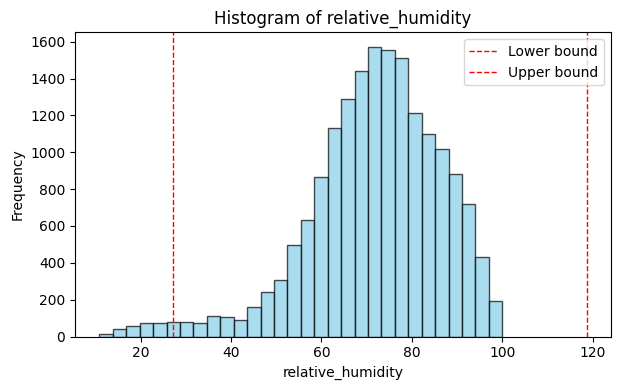
\includegraphics[width=.5\linewidth]{images/histogram_humidity.png}
    \caption{Histograma de la humedad relativa en Arona.}
    \label{histogram_1}
\end{figure}

\begin{figure}
    \centering
    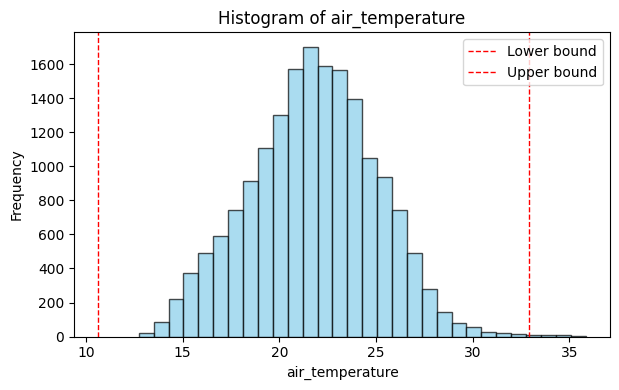
\includegraphics[width=.5\linewidth]{images/histogram_temperature.png}
    \caption{Histograma de la temperatura del aire en Arona.}
    \label{histogram_2}
\end{figure}

Por esto, se decide emplear como método de detección de anomalías el de los K vecinos más cercanos (KNN), 
una alternativa robusta que permite detectar anomalías en distribuciones no gaussianas \cite{gu2019}.

Se aplica el método de KNN a cada variable por separado, con k=10 y límite de distancia 3 veces la desviación típica.
Respecto al número de vecinos, se observa al graficar la distancia media de los K vecinos más cercanos frente a K que es poco relevante, por lo que se escoge arbitrariamente.
Una vez fijado K, para fijar el límite se considera que en una distribución gaussiana el 99,7\% de los datos se encuentran dentro de 3 desviaciones típicas y se comprueba empíricamente
este valor así como otros cercanos, observando los histogramos de valores detectados como anómalos.

Los valores anómalos son etiquetados como tales para poder ser identificados posteriormente. Se pueden observar ejemplos 
de las distancias en la figura \ref{knn_distances}. En las figuras \ref{histogram_knn_humidity} y \ref{histogram_knn_temperature} se muestran ejemplos de los valores anómalos detectados. 

Nota: Se muestran los valores anómalos indepentientemente de la variable respecto a la que se detectaron.

\begin{figure}
    \centering
    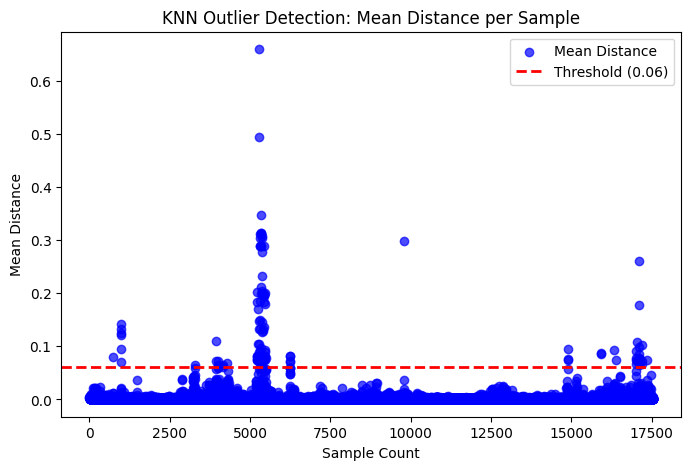
\includegraphics[width=.5\linewidth]{images/knn_distances_temperature_arona.png}
    \caption{Distancias media de los K vecinos más cercanos para la temperatura del aire en Arona.}
    \label{knn_distances}
\end{figure}

\begin{figure}
    \centering
    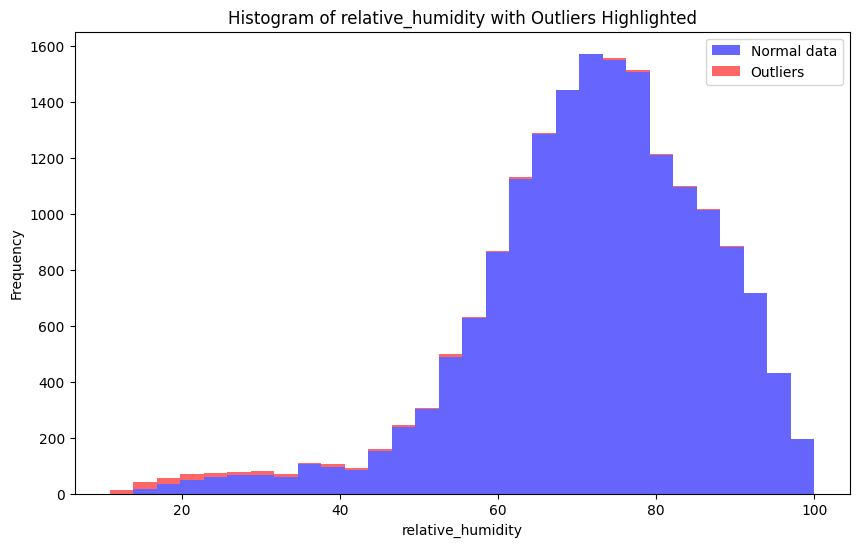
\includegraphics[width=.5\linewidth]{images/histogram_humidity_knn.png}
    \caption{Histograma de la humedad relativa en Arona con outliers detectados con knn.}
    \label{histogram_knn_humidity}
\end{figure}

\begin{figure}
    \centering
    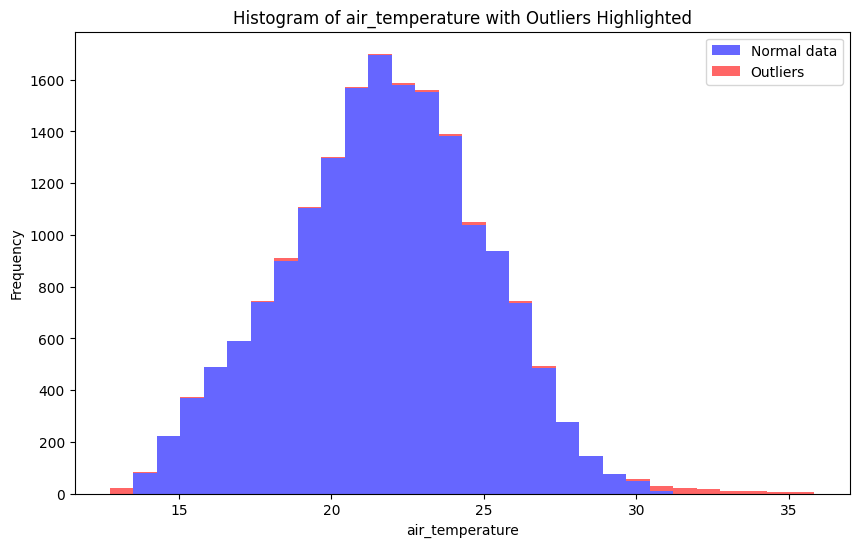
\includegraphics[width=.5\linewidth]{images/histogram_temperature_knn.png}
    \caption{Histograma de la temperatura del aire en Arona con outliers detectados con knn.}
    \label{histogram_knn_temperature}
\end{figure}

\subsection{Exploración de frecuencias - Dominio de Fourier}
Se realiza un análisis de Fourier para cada variable. De esta forma, se pueden observar las frecuencias dominantes en los datos. Este análisis
es relevante para detectar las frecuencias a emplear en la codificación de la información temporal, que se aborda en el siguiente apartado.

Se emplea la transformada rápida de Fourier (FFT), se filtran las frecuencias positivas, se acota a las frecuencias mayores a \(10^{-3}\) 
 (unos 16,66... minutos) y se grafican haciendo uso de escala logarítmica en el eje X. El pseudocódigo se muestra en \ref{fft_positive}. Se pueden observar ejemplos en las figuras \ref{fft_temperature},
 y \ref{fft_pressure}. Se señalan las 5 frecuencias de mayor magnitud con un punto en rojo. 

 \begin{figure}[H]
{\small
 \hrule \
 {\bf\small Pseudocódigo Cálculo de FFT Positiva}
 \hrule
\begin{center}
\begin{tabbing}
\ 1: {\bf Fun}\={\bf ción} calcular\_fft\_positiva($valores$, $intervalo\_muestreo$): \\
\ 2: \> \# 1. Computar la transformada rápida de Fourier del vector de entrada \\
\ 3: \> $fft\_result$ = FFT($valores$)  \\
\ 4: \> \# 2. Generar los intervalos de frecuencia para cada punto de la FFT \\
\ 5: \> $frecuencias$ = FFTFREQ(longitud($valores$), $intervalo\_muestreo$)  \\
\ 6: \> \# 3. Calcular la mitad de la longitud para aislar frecuencias no negativas \\
\ 7: \> $mitad$ = piso(longitud($valores$) / 2)  \\
\ 8: \> \# 4. Extraer solo la parte de frecuencias positivas \\
\ 9: \> $resultado\_fft\_positivo$ = $fft\_result$[0:$mitad$]  \\
\ 10: \> $frecuencias\_positivas$ = $frecuencias$[0:$mitad$]  \\
\ 11: \> \# 5. Calcular la magnitud de los coeficientes complejos resultantes \\
\ 12: \> $magnitud$ = valor\_absoluto($resultado\_fft\_positivo$)  \\
\ 13: \> \# 6. Devolver el eje de frecuencias positivas y su espectro de magnitudes \\
\ 14: \> {\bf Retornar} $frecuencias\_positivas$, $magnitud$  \\
\end{tabbing}
\end{center}
\hrule
}
\caption{Pseudocódigo Cálculo de FFT Positiva}
\label{fft_positive}
\end{figure}


\begin{figure}
    \centering
    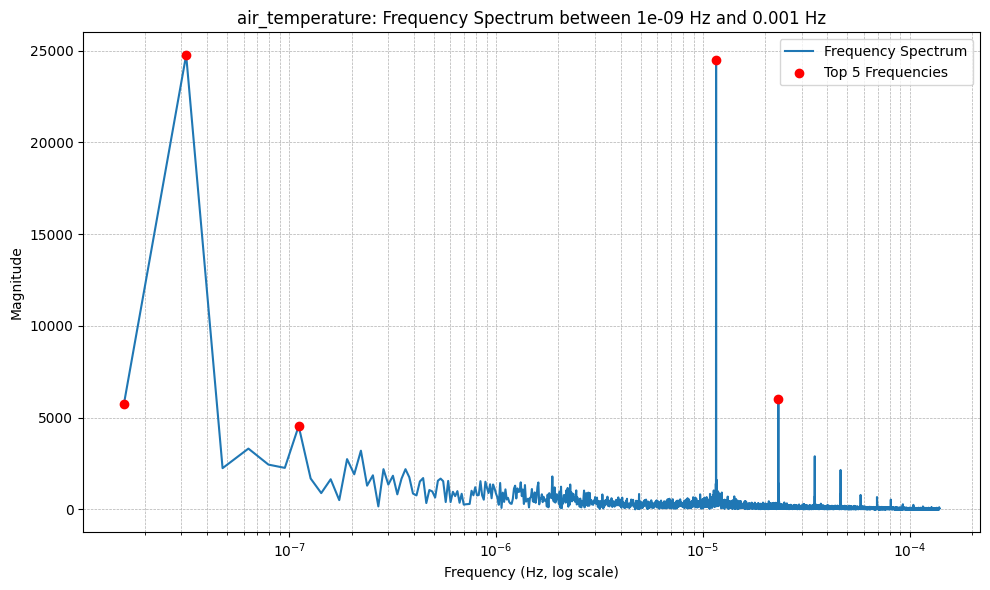
\includegraphics[width=.5\linewidth]{images/fft_temperature.png}
    \caption{Transformada rápida de Fourier de la temperatura del aire en Arona.}
    \label{fft_temperature}
\end{figure}

 \begin{figure}
    \centering
    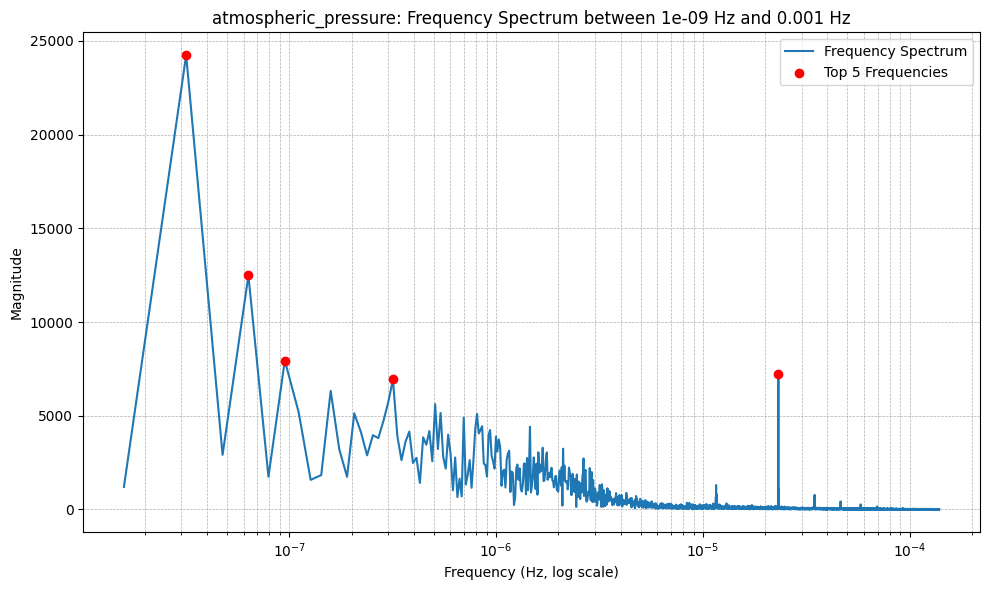
\includegraphics[width=.5\linewidth]{images/fft_pressure.png}
    \caption{Transformada rápida de Fourier de la presión atmosférica en Arona.}
    \label{fft_pressure}
\end{figure}



En la temperatura y humedad destacan las frecuencias de 24 y 8772 horas, correspondiente esta última a 365,5 días, lo que es razonable considerando que de los 
2 años de datos, uno es bisiesto. Respecto a la presión atmosférica, la más relevante es la de 12 horas, algo debido a la naturaleza de esta variable, 
que presenta este ciclo debido a un fenómeno conocido como mareas térmicas \cite{ChapmanLindzen1970}. Así mismo, la presión también presenta un pico en la frecuencia anual y la de medio año.


\subsection{Codificación de la información temporal}
Se decide codificar la información temporal mediante el uso de senos y cosenos de las frecuencias dominantes.
En base a los resultados del análisis de Fourier, se emplean la frecuencia de 24 horas y del año, teniendo especial cuidado para detectar
    si el año es bisiesto o no. De esta forma, se añaden 4 variables adicionales al dataset: sin(dia), cos(diá), sin(año) y cos(año).

Se estudia la frecuencia semanal, pero se descarta al existir poca correlación.

\subsection{Estudio de correlación}
Se estudia la correlación entre las distintas variables que conforman el dataset mediante una matriz de correlación con el coeficiente de Pearson.
Se observa que las variables climáticas tienen una correlación negativa de en torno a 0.3, lo que indica que las variables están relacionadas de 
forma baja/moderada e inversamente proporcional \ref{correlation_map}.

\begin{figure}
    \centering
    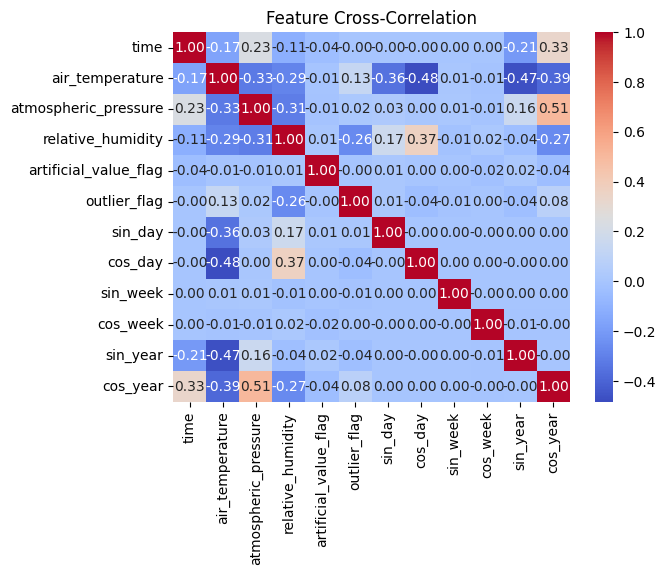
\includegraphics[width=.5\linewidth]{images/correlation_heatmap.png}
    \caption{Mapa de correlación entre las variables del dataset.}
    \label{correlation_map}
\end{figure}

\section{Creación de ventanas de datos}
Para la predicción de series temporales, los modelos neuronales requieren como entrada los valores de las variables en un número de instantes, en nuestro caso horas,
previos, que denominaremos P. Así mismo, se define un número de horas a predecir, que denominaremos N. 
De esta forma, un modelo requiere P horas de datos para predecir N horas futuras. Esto es lo que se conoce como ventana de datos.

En su versión más simple, la univariable, consta de una componente X, los valores de las variables en P pasos, y una componente Y, un vector
de tamaño N con los valores a predecir. 
No obstante, puede ser relevante incluir información adicional exógena sobre los valores a predecir, como la codificación temporal 
(o en otros dominios, si el día es festivo, etc).

De esta forma, optamos por contruir ventanas de datos con 3 componentes, X e Y, ya definidas, así como F, formada por las 4 variables de codificación temporal 
para cada paso a predecir N. Empíricamente comprobamos que la inclusión de esta información adicional mejora ligeramente el rendimiento del modelo.

En la práctica, estas ventanas se construyen mediante la técnica de ventana deslizante, que consiste en recorrer la serie temporal desplazando 
la ventana de datos en un número de pasos, que denominaremos S. Establecemos S=6 para que la ventana se desplace cada 6 horas, con el fin de evitar 
la redundancia de datos.

Como datos pasados empleamos la variable meteorológcia estudiada, así como las restantes como covariables. Se comprueba exógenamente que 
añadir estas covariables mejora el rendimiento del modelo. También se emplea como datos pasados las variables de codificación temporal. 

De esta forma, una ventana tiene X de tamaño P * 7, Y de tamaño N y F de tamaño N * 4.

\subsection{Implementación}
En primer lugar, se define una función \textit{df\_raw\_windows} que recibe como parámetros:
\itemize{
    \item df: un dataframe de pandas, que es una estructura de datos de python similar a una tabla, correspondiente a un dataset de una ubicación,
    \item P: el número de pasos pasados.
    \item N: el número de pasos a predecir.
    \item S: el número de pasos a desplazar la ventana.
    \item past\_features: un array con los nombres de las variables usadas como entradas.
    \item future\_features: un array con los nombres de las variables exógenas usadas como datos futuros.
    \item target: el nombre de la variable objetivo a predecir.
}

La función devuelve un objeto con 3 atributos,\textit{past\_variables}, \textit{future\_variables} e \textit{y}.
Siendo cada uno un arreglo con los datos de cada componente de las ventanas de datos. Es decir, la ventana i ésima
está formada por los iésimos elementos de cada uno de los 3 atributos. Esta estructura se debe al comportamiento
de las librerías de los modelos de aprendizaje profundo empleados, que procesan los datos de forma más eficiente en este formato,
como se verá más adelante.

\bigskip
El comportamiento de la función principal es el siguiente:

\begin{figure}[H]
{\small
 \hrule \
 {\bf\small Pseudocódigo Creación de Ventanas de Datos}
 \hrule
\begin{center}
\begin{tabbing}
\ 1: $train\_data$ = \{\} \\
\ 2: $test\_data$ = \{\} \\
\ 3: {\bf Par}\={\bf a cada} variable objetivo $v$: \\
\ 4: \> {\bf Par}\={\bf a cada} ubicación $u$:  \\
\ 5: \> $location\_data$ = [] \\
\ 6: \> \> {\bf Par}\={\bf a cada} dataset $d$ en la ubicación $u$:  \\
\ 7: \> \> \> $ventanas$ =  \textit{df\_raw\_windows()} \\
\ 8: \> \> \> $location\_data$.añadir($ventanas$) \\
\ 9: \> \> $windows\_count$ = len($location\_data$[0][$y$]) \\
\ 10: \> \> $overlap\_windows$ = ceil(($past\_n$ + $future\_n$)/$step$) \\
\ 11: \> \> $test\_indexes$ = random\_sample($windows\_count$, $test\_percent$) \\
\ 12: \> \> $forbidden$ = set() \\
\ 13: \> \> {\bf Par}\={\bf a cada} $index$ en $test\_indexes$: \\
\     \> \> \>   \# Prohibir el índice y las siguientes `$overlap\_windows$ - 1` ventanas \\
\ 14: \> \> \>   {\bf Par}\={\bf a cada} \= $j$ en rango($overlap\_windows$): \\
\ 15: \> \> \> \>     $forbidden$.add($index$ + $j$) \\
\ 16: \> \> $train\_indexes$ = rango($windows\_count$) - $forbidden$ \\

\ 17: \> \> {\bf Par}\={\bf a cada} dataset $d$ en $location\_data$: \\
\ 18: \> \> \> $past\_variables\_windows$ = $location\_data$[$d$]["past\_variables"] \\
\ 19: \> \> \> $future\_variables\_windows$ = $location\_data$[$d$]["future\_variables"] \\
\ 20: \> \> \> $y\_windows$ = $location\_data$[$d$]["y"] \\
\     \> \> \> \# Construcción de conjuntos de entrenamiento y validación \\
\ 21: \> \> \> $train\_past\_variables$ = [$past\_variables\_windows$[i] para i en $train\_indexes$] \\
\ 22: \> \> \> $train\_future\_variables$ = [$future\_variables\_windows$[i] para i en $train\_indexes$] \\
\ 23: \> \> \> $train\_y$ = [$y\_windows$[i] para i en $train\_indexes$] \\

\ 24: \> \> \> $test\_past\_variables$ = [$past\_variables\_windows$[i] para i en $test\_indexes$] \\
\ 25: \> \> \> $test\_future\_variables$ = [$future\_variables\_windows$[i] para i en $test\_indexes$] \\
\ 26: \> \> \> $test\_y$ = [$y\_windows$[i] para i en $test\_indexes$] \\
      
\ 27: \> \> \> $train\_data$[$v$]["past\_variables"].extender($train\_past\_variables$) \\
\ 28: \> \> \> $train\_data$[$v$]["future\_variables"].extender($train\_future\_variables$) \\
\ 29: \> \> \> $train\_data$[$v$][\string"y"].extender($train\_y$) \\
        
\ 30: \> \> \> $test\_data$[$v$]["past\_variables"].extender($test\_past\_variables$) \\
\ 31: \> \> \> $test\_data$[$v$]["future\_variables"].extender($test\_future\_variables$) \\
\ 32: \> \> \> $test\_data$[$v$][\string"y"].extender($test\_y$) \\

\end{tabbing}
\end{center}
\hrule
}
\caption{Pseudocódigo Creación de Ventanas de Datos}
\label{branch_and_bound_max_diversity}
\end{figure}

Para cada ubicación se eligen los índices de las ventanas de test aleatoriamente. Estos índices son los mismos para los dos datasets de una localización, 
puesto que los datos son bastante similares entre ambos y queremos evitar el filtrado de información. 
Cabe destacar la consideración de ventanas "prohibidas", que se descartan del conjunto de entrenamietno para evitar filtrar datos.
De esta forma, todas las ventanas previas que estén solapadas con una ventana de test son descartadas.

\subsection{Normalización}
Se utilizan las ventanas del conjunto de entremaniento para calcular las características de la normalización.
Usamos la estandarización o normalización Z-score, que consiste en restar la media y dividir por la desviación típica.
De esta forma, los datos quedan centrados en 0 y con una desviación típica de 1.

La normalización se aplica a la variable objetivo y las covariables meteorológicas, tanto en los datos pasados como los datos a predecir ($y$). 
No se aplica a las variables de codificación temporal, ya que al tratarse de senos y cosenos, su rango ya es limitado entre -1 y 1.

Debemos almacenar los parámetros de normalización puesto que serán necesarios para tratar cualquier dato que se suministre en el futuro al sistema.
